\documentclass{sig-alternate}

\usepackage[utf8]{inputenc}
\usepackage[hyphens]{url}
\usepackage[pdftex,urlcolor=black,colorlinks=true,linkcolor=black,citecolor=black]{hyperref}
\def\sectionautorefname{Section}
\def\subsectionautorefname{Subsection}
\usepackage{graphicx}
% todo macro
\usepackage{color}
\newcommand{\todo}[1]{\noindent\textcolor{red}{{\bf \{TODO}: #1{\bf \}}}}

\title{From Freebase to Wikidata: The Great Migration}

\numberofauthors{3}
\author{
Thomas Pellissier Tanon,\titlenote{The author was an intern at Google when the majority of the work was done.}\ Denny Vrandečić\\
   \affaddr{Google, San Francisco, United States of America}\\   
   \email{\{thomaspt, vrandecic\}@google.com}
\alignauthor
Sebastian Schaffert\\
   \affaddr{Google, Zurich, Switzerland}\\   
   \email{schaffert@google.com}
\alignauthor
Thomas Steiner\\
   \affaddr{Google, Hamburg, Germany}\\   
   \email{tsteiner@google.com}
}

\begin{document}

\maketitle

\begin{abstract}
Collaborative knowledge bases that make their data available in machine-readable form
as structured data are central to many companies' data strategies.
One example of such collaborative knowledge bases is Freebase (\url{www.freebase.com}),
created with proprietary technologies in 2007 by a~company called Metaweb,
which was then acquired by Google in 2010.
Another example is Wikidata (\url{www.wikidata.org}),
a~collaborative knowledge base developed in the open since 2012 by Wikimedia Deutschland
and operated by the Wikimedia Foundation.
Due to the success of Wikidata, Google decided to shut down Freebase and
help with the transfer of its content to Wikidata through a~crowdsourcing approach.
In this paper, we describe the ongoing transfer efforts and challenges,
and provide an analysis of the process so far.
\end{abstract}

% a~category with the (minimum) three required fields
\category{H.4}{\todo{Hierarchy}}{Miscellaneous}

\terms{\todo{Terms}}

\keywords{\todo{Keywords}}

\section{Introduction}

Moving data between two knowledge bases that do not share a~similar design
is usually a~problematic task and requires the careful mapping between their structures.
In this paper, we describe how we facilitated the migration of Freebase content to Wikidata.
That migration was no exception to this rule, and had a~number of \emph{structural} challenges.
Even more challenging was the \emph{cultural} difference between the two involved communities.
The Freebase and Wikidata communities have a~very different background,
subtly different goals and understandings of their tasks,
and different requirements regarding their data.
\todo{Expand}

The remainder of this paper is structured as follows.
After an introduction to the two collaborative knowledge bases
Freebase and Wikidata in \autoref{sec:background},
we describe our methodology and the metrics used to measure the migration
in \autoref{sec:challenges-of-the-migration}.
In order to support the migration, we have developed a~set of open source tools
that we present in \autoref{sec:primary-sources-tool}.
We then present the results of the migration
and discuss these statistics in \autoref{sec:statistics-of-the-migration}.
The paper terminates with an outlook at proposed next steps
and a~conclusion in \autoref{sec:future-work-and-conclusion}.

\section{Background}\label{sec:background}

\subsection{Freebase}

Freebase\footnote{Freebase: \url{https://www.freebase.com/}} is an open source and
collaborative knowledge base created in 2007 by Metaweb and acquired in 2010 by Google.
It was used as the open core of the Google Knowledge Graph,
and also has many use cases outside of Google.

Due to the success of Wikidata,
it was decided to close Freebase and support the migration of its contents to Wikidata.
Freebase relies on the notions of \emph{topics}, \emph{facts}, \emph{types}, and \emph{properties}.
Each Freebase topic has a~stable identifier called \emph{``mid''} (for Metaweb ID),
one or more types, and uses properties from these types in order to provide facts.
For example, the Freebase topic for Barack Obama has the mid \texttt{/m/02mjmr}
and the type \texttt{/government/us\_president} that allows the entity to have
a fact with the property \texttt{/government/us\_president/presidency\_number}
and the literal integer ``44'' as the value.

\begin{figure}[!htbp]
\centering
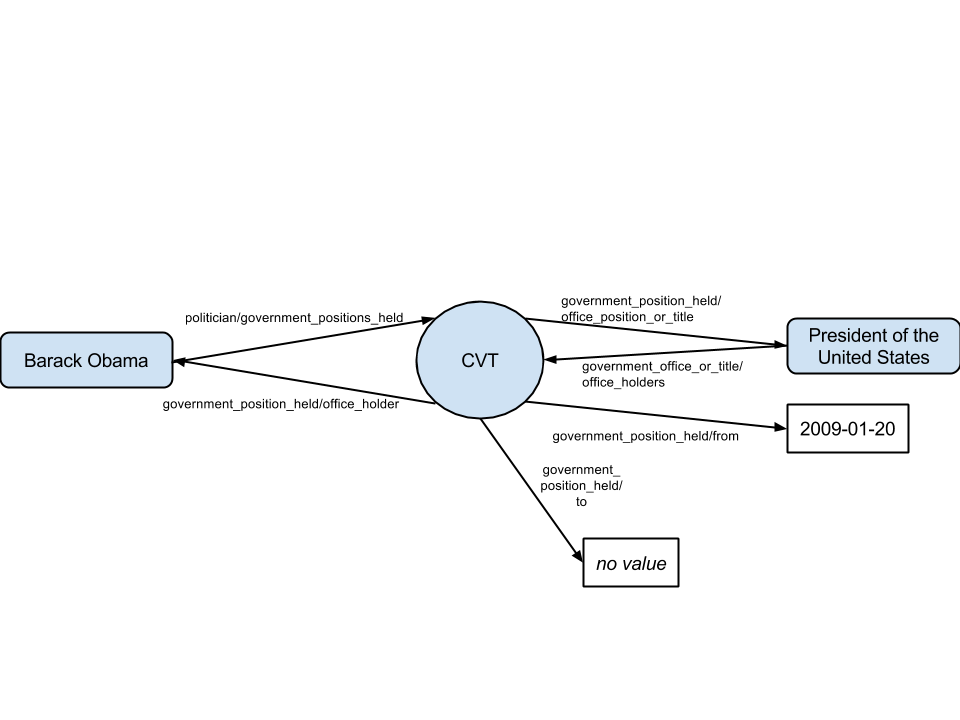
\includegraphics[width=8.45 cm]{img/freebase-cvt-obama.png}
\caption{\todo{Crop, get PDF version} Example of CVT: presidency of Barack Obama}
\label{fig:cvt-obama}
\end{figure}

To represent complex values like geographic coordinates or to annotate relations,
for example, in order to add start and end dates for a~position held,
Freebase has introduced the notion of Compound Value Types (CVTs, see \autoref{fig:cvt-obama}).
They behave like topics, \emph{e.g.}, have a~mid and can have types,
but do not have the \texttt{/common/topic} type.

The contents of Freebase have been imported from various sources like Wikipedia
or the Internet Movie Database IMDB,
in consequence Google does not own the copyright of some parts of the contents of the knowledge base
like images or long entity descriptions extracted from Wikipedia.
As of the closing of Freebase on March~31, 2015,
it counted more than 3~billion facts about almost 50M~entities.

\subsection{Wikidata}

Wikidata\footnote{Wikidata: \url{https://www.wikidata.org/wiki/Wikidata:Main_Page}}
is a~collaborative knowledge base
launched in October 2012 and hosted by the Wikimedia Foundation.
Its community has been growing quickly since the beginning, and as of mid 2015,
the community comprises about 6,000 active contributors.

Wikidata contents rely on the notions of \emph{item} and \emph{statement}.
An item represent a~concept, has a~stable identifier and may have some labels,
descriptions, and aliases in multiple languages, links to pages about this concept
in the others Wikimedia projects, like Wikipedia, and statements.
Contrary to Freebase, Wikidata encodes with its statements not true facts,
but \emph{claims} from different sources.

A~statement is composed of one claim and zero or more references for this claim.
The claim itself is composed of one main property--value couple that encodes
the main (claimed) fact like ``population is 8,173,900'' and optional qualifiers
to add information about it like ``as of June 2012''.
\autoref{fig:statement} illustrates the used nomenclature with an example.

The contents of Wikidata are freely available under a~Creative Commons~0 (CC0) license.
As of mid 2015, Wikidata counted about 66M~statements on 14M~entities.
For more background information about Wikidata, see~\cite{vrandevcic2014wikidata}
by Vrandečić and Krötzsch.
For a~comparison between Freebase and Wikidata,
we refer the reader to~\cite{farbercomparative} by Färber \emph{et~al.}

\begin{figure}[!htbp]
\centering
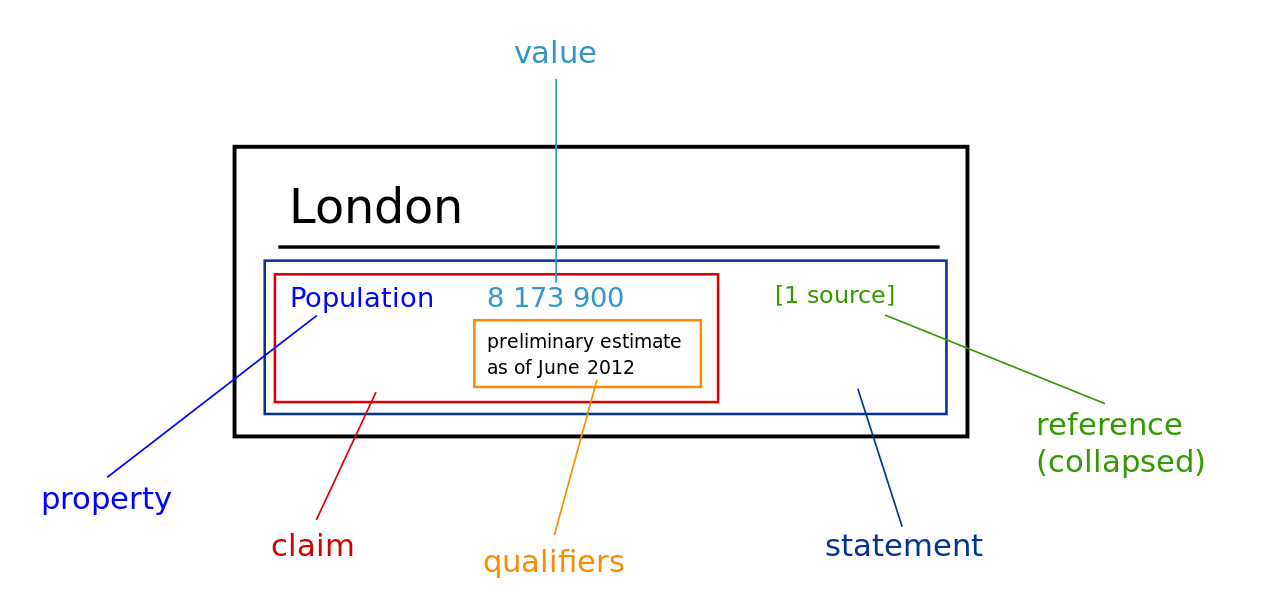
\includegraphics[width=8.45 cm]{img/Wikidata-statement.png}
\caption{\todo{Get PDF version} An example of Wikidata statement (from
	\url{https://commons.wikimedia.org/wiki/File:Wikidata_statement.svg})}
\label{fig:statement}
\end{figure}

\section{Challenges of the migration}\label{sec:challenges-of-the-migration}

Migrating data from Freebase to Wikidata faced a~number of challenges:

\subsection{Licensing}
\label{sec-licensing}

The first challenge is regarding the licenses under which the datasets are published.
Wikidata is published under a~Creative Commons~0 (CC0) license (similar to the public domain),
while Freebase is under a~Creative Commons By license and contains data
imported from external projects not owned by Google,
like images or descriptions extracted from Wikipedia.
In a~first step we filtered the Freebase dump from this kind of content
before being able to have a~dump that Google could relicense under CC0.
This step reduces the number of republishable Freebase facts by about 42M~facts.

\subsection{References}

The second challenge is that the Wikidata community is very interested to have references
for their statements, sources that Freebase usually did not store except for
some specific data like populations and unemployment rates.
For these two specific cases we have just kept the references from Freebase.
In order to provide the Wikidata community with references for the facts in Freebase
we have reused data from the Knowledge Vault, another Google project with the aim
to extract facts from the web (see~\cite{dong2014knowledge}).
Whereas the fact extraction was usually correct, the pages Knowledge Vault extracted
the references from often do not meet the requirement for a~good reference:
they include pages in social networks, shopping sites, filesharers, \emph{etc.}
It became necessary to filter and curate the references before inclusion in Wikidata.

\subsection{Data Quality}

The quality of the data in Freebase was challenged by the Wikidata community.
For example, a~small city in France had an ISO country code%
\footnote{See \url{http://www.freebase.com/m/03cc0d0}}.
Another example, Boston (the city in Massachusetts) has the type \texttt{/people/person}.
A fully automatic upload of all the content from Freebase into Wikidata
did not seem advisable as the expectations of the community regarding
the quality of the content automatically added to Wikidata are high (and rightly so).
Also, whereas an upload of all the data might have lead to accelerated growth
in the short term, such a~fast upload might also endanger the sense of ownership
the Wikidata community has for its data.
Instead we decided to rely on human curation and created Primary Sources,
a simple tool which displays statements to the user that may be added to the currently shown item.
The user can, with only one click, reject the statement or approve it and save it to Wikidata.
It is currently available as a~gadget, an opt-in option in Wikidata.
This tool has no dependencies on Freebase and may be easily reused by other projects
which may want to import data into Wikidata.
For that we have implemented an upload API and a~feature that allows users
to display only statements from a~given dataset.
In fact, during the project one other researcher approached us in order to upload
a dataset extracted from natural language text.
A statistics dashboard has also been created in order to monitor the curation work
\url{https://tools.wmflabs.org/wikidata-primary-sources/status.html}
and the source code of the tool is available on GitHub:
\url{https://github.com/google/primarysources}.

\begin{figure}[!htbp]
\centering
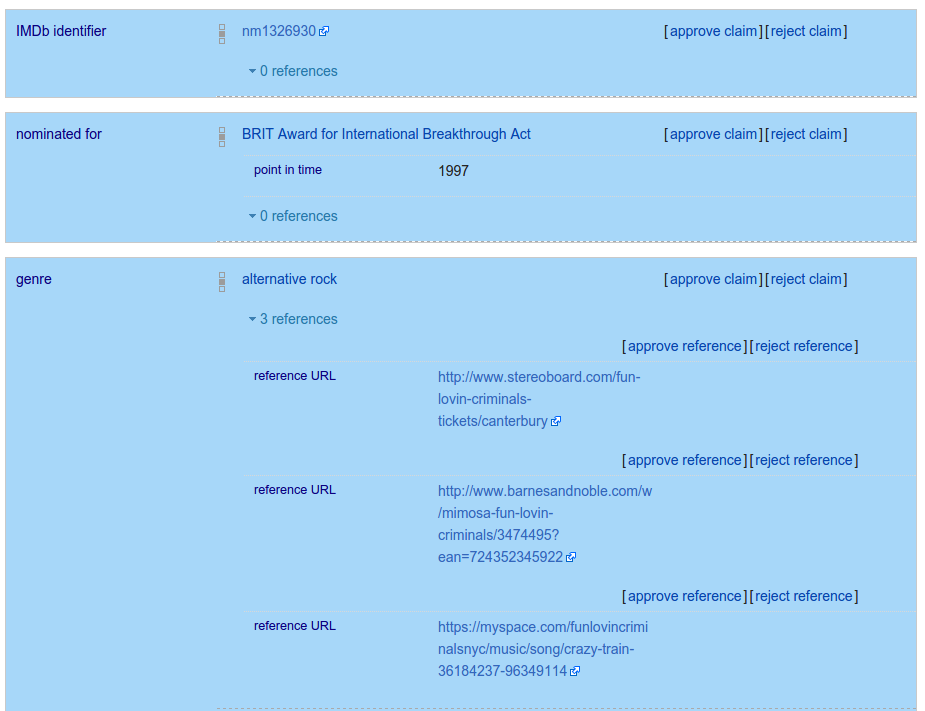
\includegraphics[width=8.45 cm]{img/primary-sources.png}
\caption{Primary Sources user interface}
\end{figure}

Currently (August~18, 2015) the tool has been used by more than a~hundred users
who have performed more than 15,000 approve or reject actions.
More than 12M~statements are uploaded to the tool.

\subsection{Mappings}

\subsubsection{Mappings of Items}

Another challenge is to get a~good mapping between Freebase topics and properties
and Wikidata items and properties.
Two mappings between Freebase topics and Wikidata items were initially available,
and we worked on further mappings.
A first one has been created by Google in October 2013%
\footnote{Freebase mappings \url{http://developers.google.com/freebase/data}}
and is based on Wikipedia links already present in Freebase: if a~Freebase topic and
a Wikidata items share at least two Wikipedia links, then they are about the same subject.
The quality of this mapping is considered as very good by the Wikidata community
who have uploaded it to the wiki and further curated and maintained it by hand.
It maps 1.15M~of Freebase topic.
A second mapping has been created by Samsung, and is actively maintained%
\footnote{Samsung mappings \url{http://github.com/Samsung/KnowledgeSharingPlatform}.}.
It is based on the same idea but matches a~Freebase topic with a~Wikidata item
even if there is only a~single Wikipedia link shared.
The quality of the mapping is lower (there are some wrong matches,
often because there is no clear separation between topics and disambiguation pages in Wikipedia)
but it provides 4.4M~links.
As we have seen before, our quality target is not very high,
so we have chosen to merge the two dumps and, for the 6,000 conflicts,
to prioritize the mapping given by Wikidata.
To improve the resulting mapping we have also tried to do some reconciliation
based on external database IDs shared by Freebase and Wikidata, like MusicBrainz, VIAF, \emph{etc.}
With this technique we were able to match 0.8M~IDs,
creating a~mapping for 0.6M~topics---most of them already in our dataset.
This resulted in an additional 84,000 items mapped.
We also used data from Google's Knowledge Graph to add 0.1M~further mappings
matching also a~topic and an item if they share a~Wikipedia link.
We could maybe add some more data by looking at functional relations like ``father'' and ``mother''.
But these relations only apply to relatively small sets of data (like well known families)
and the functional assumption may run into some edge cases.
For example, the \texttt{/people/person/parents} property in Freebase also covers also stepparents,
creating cases where a~person has more than one male or female \texttt{/people/person/parents}.
Eventually, with these four sources we mapped 4.56M~items.
We believe that by doing so we have mapped most of the topics that could be automatically mapped
as suggested by the small increases added by the ID reconciliation approach
and the Knowledge Graph data.
Furthermore, the mapped topics have an average number of facts of about~13.9,
whereas the topics that were not mapped have an average of 5.7~facts.
We have mapped the majority of topics with more than 80~facts.
This allows us to conclude that we have mapped the most important items of Freebase.

\begin{figure}[!htbp]
\centering
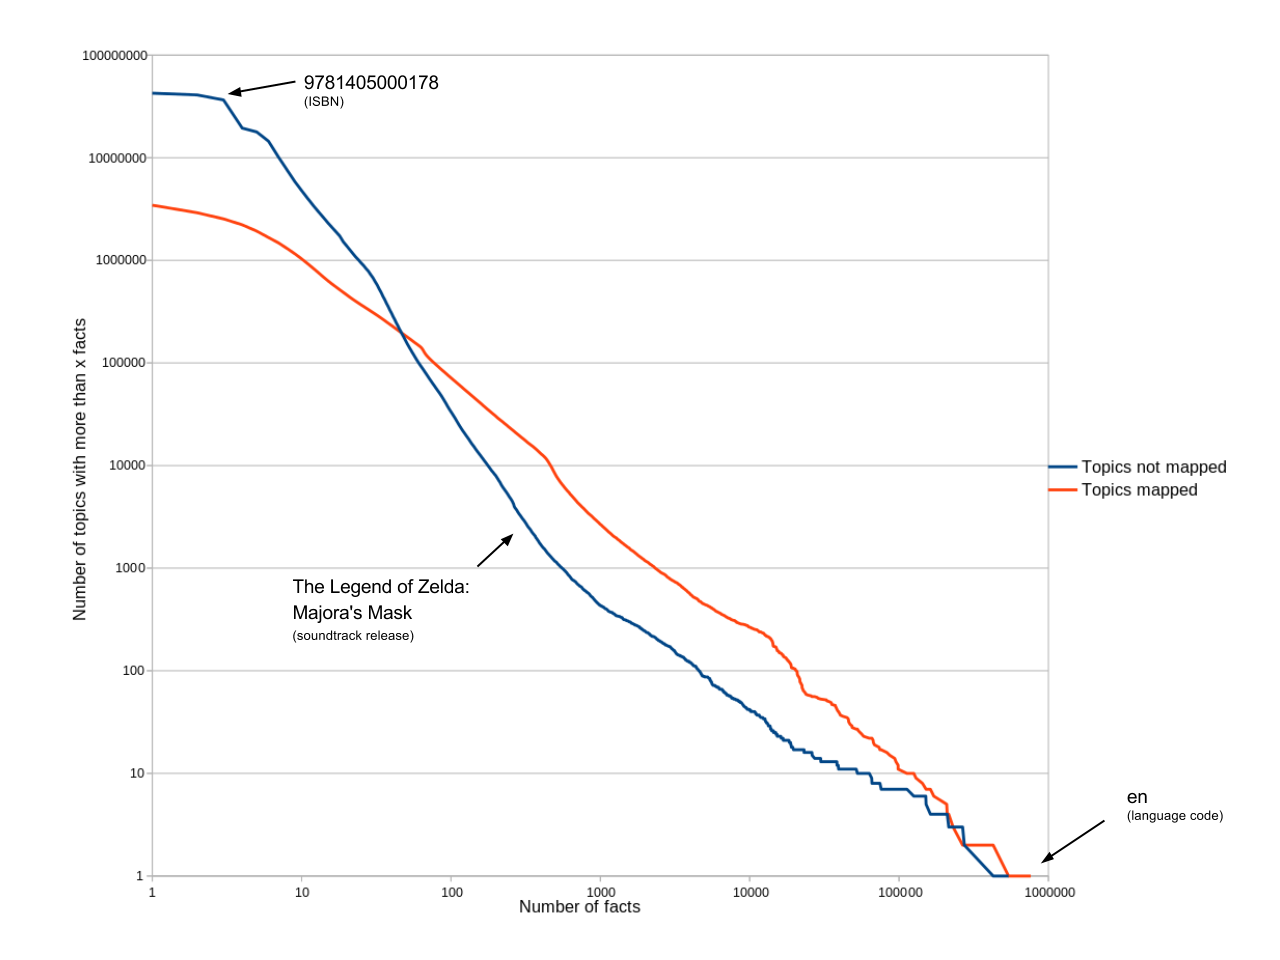
\includegraphics[width=8.45 cm]{img/facts-topics-mapping.png}
\caption{Number of mapped and not mapped topics with more than x facts.
Note the log scale on both axis.}
\end{figure}

\subsubsection{Mapping of Properties}

For the mapping between Freebase and Wikidata properties we have chosen to do it by hand
with the help of the Wikidata community.
With that we have been able to map quickly around 360~properties
(note that Wikidata has a~total of 1,660 properties, and Freebase has around 37,700 properties).
For the mapping of properties where the domain are other topics or literals
this mapping provides the Wikidata property to use.
We have also implemented a~special case for \texttt{/people/person/parents}
in order to be able to map them to Wikidata properties ``father'' and ``mother''
based on the person gender.
The mapping of CVTs is more complicated because it is not possible to have a~1~to~1 relationship
between Freebase and Wikidata properties: the CVT is linked to the subject topic by one property
and has properties pointing to its component values, whereas the Wikidata statement
has a~main property value group that is qualified by other such groups.
In order to map a~CVT to a~statement, we have to know which of the CVT's properties
should be used as the main value of the statement, with the others being mapping to qualifiers.
In order to keep a~simple mapping associating one Wikidata property to one Freebase property,
we map both the property linking the topic to the CVT
and the main property of the CVT to the same Wikidata property, and, during the mapping process,
we pick the later as the main property of the CVT.
For example, if we try to map the same CVT as \autoref{fig:cvt-obama}
we will use the Wikidata property ``position held (P39)'' to map
\texttt{/politician/government\_positions\_held} and
\texttt{/government\_position\_held/office\_position\_or\_title}, use ``start time (P580)''
for \texttt{/government\_position\_held/from} and ``end time (P582)'' for
\texttt{/government\_position\_held/to}.
With this mapping the created Wikidata statement will be
like the one presented in \autoref{fig:statement-obama}.

\begin{figure}[!htbp]
\centering
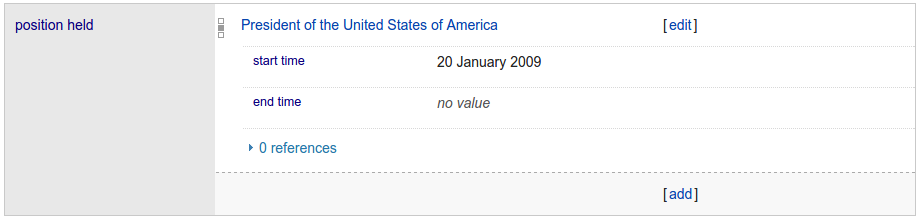
\includegraphics[width=8.45 cm]{img/wikidata-statement-obama.png}
\caption{Target Wikidata statement}
\label{fig:statement-obama}
\end{figure}

For CVTs that include sources, we map the property that links the CVT
to the source as a~Wikidata reference instead of a~qualifier.
The last challenge is to do the real mapping, taking care of CVTs
and the complex datatypes of Wikidata.
For CVTs, when we have a~triple whose value is a~CVT, we just retrieve it,
map all its component triples (while ignoring ones that can't be mapped)
and apply the above mechanism to get its main value.
For values, we use the datatype information stored with Wikidata properties
in order to cast values to the right type.
For quantities we assume that the amounts are precise
as there is no precision information in Freebase.
For globe coordinates we have hardcoded the mapping of the \texttt{/location/geocode} CVT
into the globe-coordinate value type of Wikibase
and use the same precision guess algorithm as the one used by Wikidata user interface.
For dates we just map the date and time values (encoded using XSD%
\footnote{\url{ http://www.w3.org/TR/xmlschema11-2/}} types)
to the Wikidata ``time'' datatype but we filterout dates before 1920 that have
a higher precision than year because we do not know
if there are in Julian or Gregorian calendar and so,
we are not able to fill the ``calendar'' metadata of the Wikidata ``time'' datatype.

\section{Primary Sources Tool}\label{sec:primary-sources-tool}

\subsection{Data Preparation}

\todo{Denny: write me}

\subsection{Back-end of the Tool}

\todo{Sebastian: write me}

\subsection{Front-end of the Tool}

\todo{Tom: write me}

\section{Statistics on the Migration}\label{sec:statistics-of-the-migration}

Here is an overview of the size of the last dump of Freebase:

\begin{itemize}
  \setlength\itemsep{0em}
  \item 48M~topics
  \item 2,997M triples
  \item 442M facts owned by Google\footnote{These ``facts'' are the Freebase triples
      after having filterout the data about ids (\texttt{/type/object/id}),
      types (\texttt{/type/object/type}), labels and descriptions (\texttt{/type/object/name},
      \texttt{/common/topic/description}...) and triples that should be filtered
      for legal reasons (see \autoref{sec-licensing}).}
  \item 68M~labels
\end{itemize}

To compare, Wikidata contains (as of August 2015):

\begin{itemize}
    \setlength\itemsep{0em}
    \item 14.5M~items
    \item 66M~statements
    \item 82M~labels
\end{itemize}

But why are these numbers so different?
Regarding the number of topics, Freebase has a~lot of topics about subjects
that do not match the Wikidata notability criteria%
\footnote{\url{https://www.wikidata.org/wiki/Wikidata:Notability}}.
For example, Freebase has 11.3M~musical recordings, 8.3M~music canonical versions,
2.6M~ISBNs, \emph{etc.}
We also cannot compare the number of facts and the number of statements directly,
even considering the lower number of topics.
Freebase encodes its knowledge in far many more facts than Wikidata needs statements.
Properties in Freebase often have a~reverse property used in order to be able
to traverse the Freebase graph easily in both directions.
For example the property \texttt{/people/person/place\_of\_birth} will have as reverse
the property \texttt{/location/location/people\_born\_here} that encodes
exactly the same semantic information.
Such reverses sometimes exist in Wikidata (like ``children'' for ``father'' and ``mother'')
but are far less common.
Another point is that CVTs use a~lot of facts to tell the same thing that
would be represented by a~single Wikidata statement.
For example, to encode that Barack Obama is the president of the United States from June~20, 2009,
Freebase requires more than six facts as shown in \autoref{fig:cvt-obama}.
If we try to encode Wikidata statements as if they were Freebase facts, \emph{i.e.},
by removing sources, representing statements with qualifiers using CVTs
and adding reverse properties it would lead to 110M of facts,
\emph{i.e.}, 167\% of the raw number of statements.
Sometimes, Freebase contains also duplicate data.
For example, a~lot of cities in the United States have duplicate CVTs for the population
where the only change is the encoding of the source
%\footnote{See, for example, \url{http://www.freebase.com/m/01jr6}.}.

\begin{figure}[!htbp]
\centering
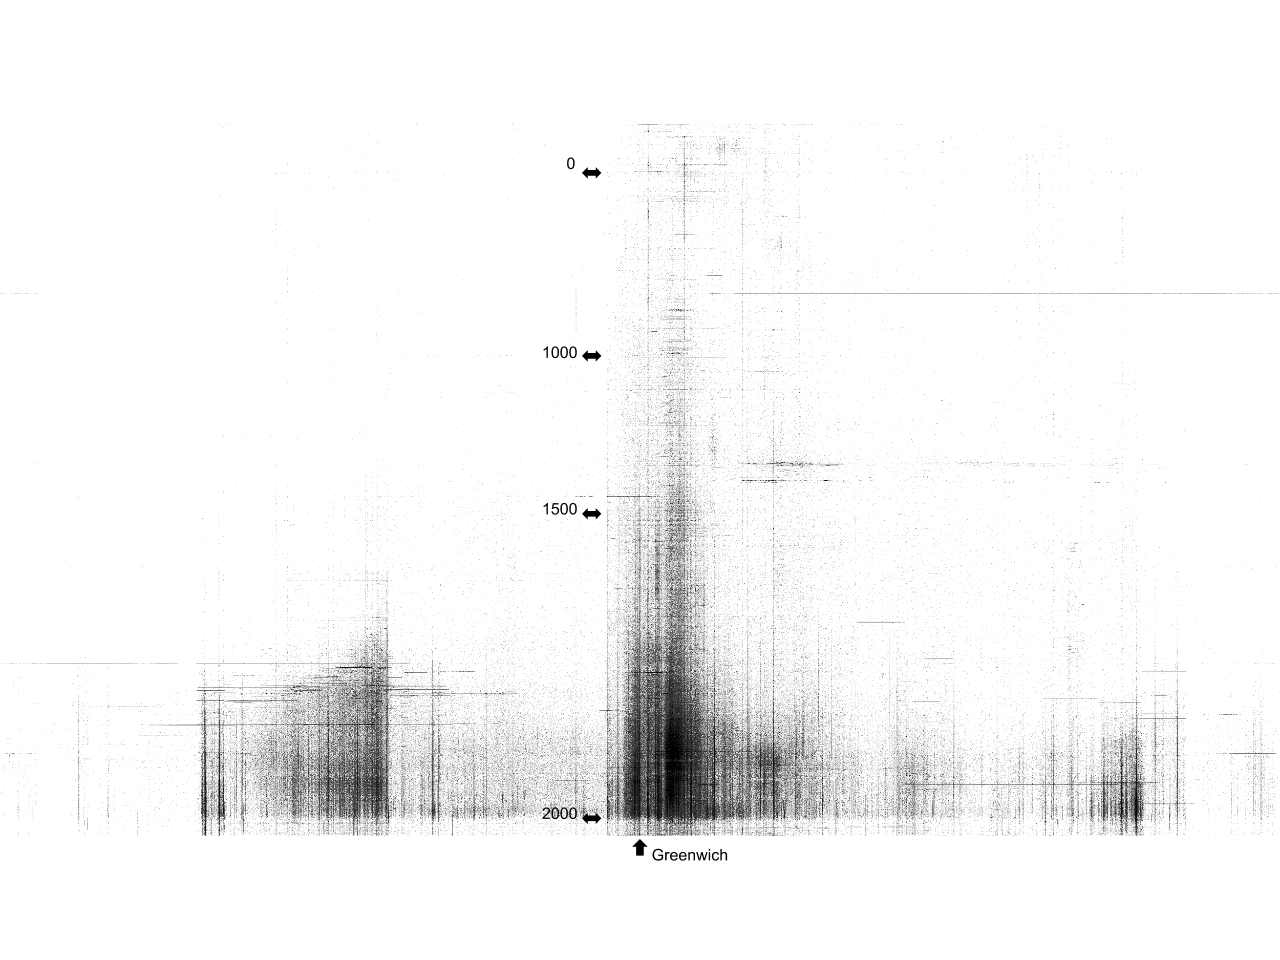
\includegraphics[width=8.45 cm]{img/wikidata-time-space.png}
\caption{Time and spatial distribution of Wikidata items.
Longitude is in $x$ axis and time, following a~power law ($y' = y^8$), is in $y$ axis}
\label{fig:time-space-wikidata}
\end{figure}

\begin{figure}[!htbp]
\centering
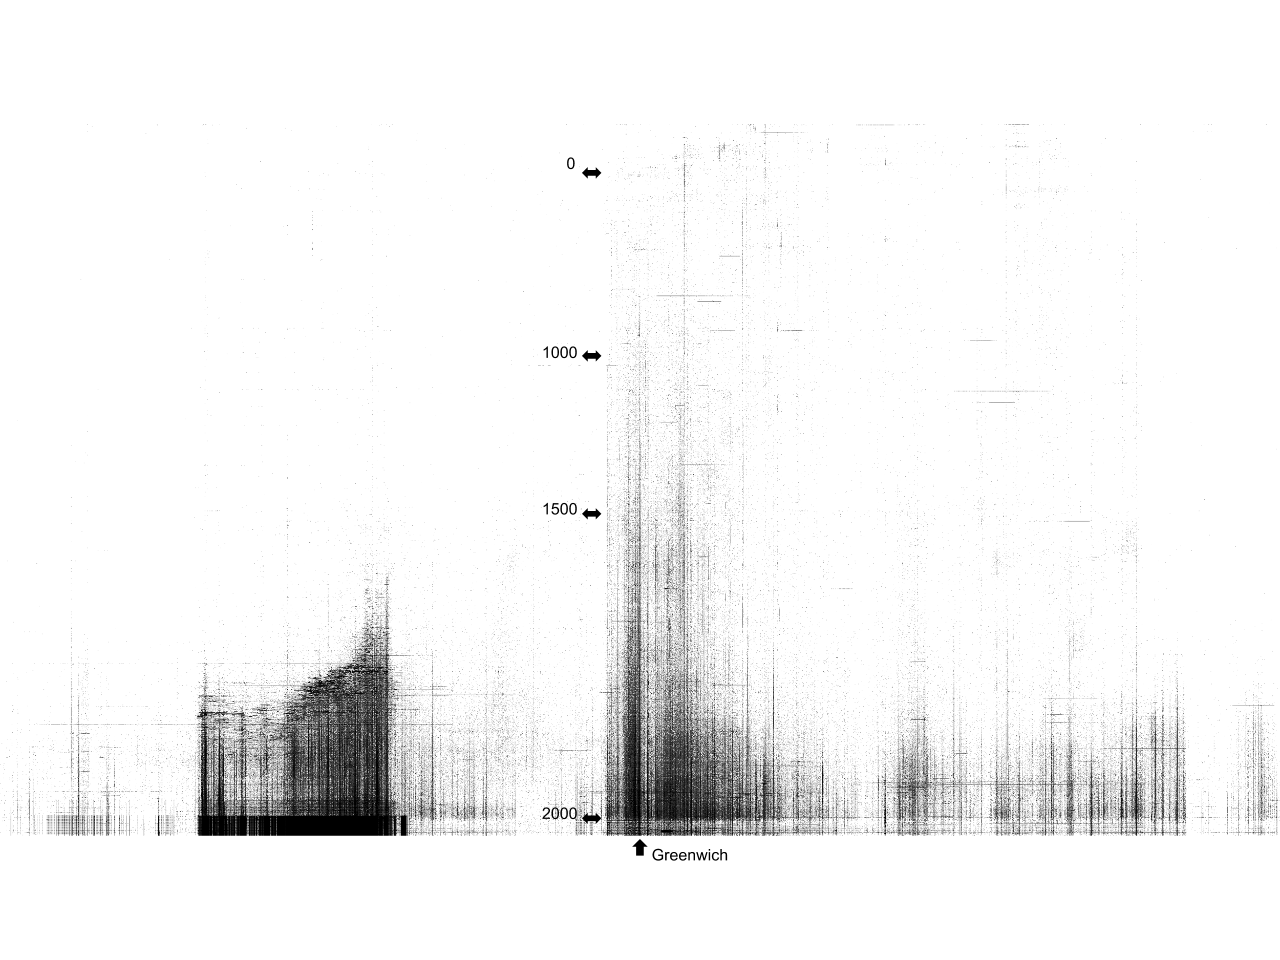
\includegraphics[width=8.45 cm]{img/freebase-time-space.png}
\caption{Same figure for Freebase entities}
\label{fig:time-space-freebase}
\end{figure}

We have also created a~time-spatial visualization of Freebase and Wikidata in order
to get an idea of the coverage of the two knowledge bases
(see \autoref{fig:time-space-wikidata} and \autoref{fig:time-space-freebase}).
The used method is to extract the earliest date and the longitude
linked to each knowledge base entities
and propagate them to the connected entities which do not have such data
using a~decreasing exponential distribution.
We see that the two knowledge bases follow the same basic patterns,
with a~coverage mostly concentrated on Europe and North America,
and there are no strong differences between them.
The coverage of the after 2000 entities seems better in Freebase, maybe because of
the presence of a~lot of musical data missing in Wikidata and of the U.S.
population CVTs.
The big horizontal lines seems to be mostly due on places that do not have any linked date
and so inherit the foundation date of their country.
For Wikidata, two lines that are caused by this behavior are the big line over the U.S.A around 1780
and the one covering Russia around 850.
We could conclude from this visualization that Wikidata, even with its smaller size,
seems to have a~nearly as good coverage of the world as Freebase.
To conclude, it is tricky to find good ways to compare the two databases
and good metrics of success for the migration and we could state that, for a~knowledge base,
containing far more triples than the other does not mean
it contains the same proportion of additional good data.

\subsection{Raw Statistics}

From the Freebase dump we have been able to create more than 17M~Wikidata claims
(\emph{i.e.}, statement without references) including 1.5M~IDs.
For that we have used 31M~facts.
When we add some references we get 19.6M~statements, and, after removing 1M~of duplicates
and the ones already in Wikidata, we obtain 14M~new statements.
So, if all these statements were added to Wikidata,
it would lead to a~21\% increase of Wikidata statements number.
But why are these numbers so low compared to the size of Freebase?
We believe that the main reason is that we have only mapped to Wikidata 4.56M~items, (\emph{i.e.},
only 9.5\% of Freebase topics), that are the subject of only 64M~facts.
So, we could not hope to map more than 64M~statements
assuming that we could map all reverse properties, and we couldn't.
So, assuming that we do not care about the not mapped topics,
we have created a~statement for more than 24\% of the facts.
If we restrict ourselves to the reviewed facts, a~set of 1.6M~facts
that have been human curated, we have far better results.
There are 0.58M~facts which subjects are mapped to Wikidata and 0.52M~of them
(\emph{i.e.}, 92\%) are converted into Wikidata statements.
And we would get another 1\% if we would be able
to map the properties \texttt{/people/person/weight\_kg}
and \texttt{/people/person/height\_meters} that Wikidata are not supporting yet.
58\% of the statements created from reviewed fact are already in Wikidata,
allowing us to add 0.25M~of new reviewed statements to Wikidata.

\section{Future Work and Conclusion}\label{sec:future-work-and-conclusion}

We believe that the main way of improvements is to extend the migration to more Freebase topics
by suggesting Wikidata users to create new Wikidata items.
A possible way of doing it is to create a~small gamified user interface that would allow users
to create new Wikidata items for a~suggested topic or to add map them to an existing Wikidata item.
In order to suggest interesting topics to add to Wikidata
we could rank the not mapped yet topics per number of incoming links from already mapped topic
and filter not interesting types like ISBNs.
Another way of improvement is to upload using a~bot high quality datasets,
like the reviewed facts or some sets,
for external ids in order to speed up the integration of Freebase content into Wikidata.
We have already started to upload the simple reviewed facts about humans
like birth date, death place or gender using a~bot.
We have also started to investigate on importing some labels
that are in Freebase and are missing in Wikidata.
In the 17.2M~of Freebase labels for mapped topics only 0.9M, \emph{i.e.},
5\%, are missing in Wikidata.

We have been able in a~fairly short amount of time to provide to the Wikidata community
more than 14M~of new Wikidata statements using a~new tool
well integrated into the Wikidata user interface.
The effort needed to map two fairly different knowledge bases has also been a~good occasion
to highlight the difficulty to have good metrics to measure the size
and, so, the ``value'', of such databases.
We hope that this project will allow to increase the completeness of Wikidata and,
helped by the comparison to another database, to improve its quality.

\bibliographystyle{abbrv}
\bibliography{biblio}

\balancecolumns
\end{document}
